\documentclass[main.tex]{subfiles}
\begin{document}
\chapter{Introduction}
The standard model of particle physics (SM) is our current best working
theory that describes the phenomenon we observe, for  example,
 at collider experiments.
The large hadron collider (LHC) is a high energy proton-proton
collider experiment that allows us to study the fundamental particles
laid out in the standard model.

The interaction of these fundamental particles are described
by scattering amplitudes. The standard model allows us to
calculate these amplitudes, or matrix elements, from first
principles. A key challenge in the past few decades has been
to compute these matrix elements for increasing number of
final state particles and for higher orders in perturbative
expansations in fixed order calculations. Although there
has been tremendous progress in this sector a complication
that naturally arises is that the evaluation of these matrix
elements becomes increasingly time consuming due to their
algebraic complexity.

The topic of this thesis is to apply modern machine learning
techniques to reduce the time spent evaluating these
complex matrix elements. Considering the physical properties
of these matrix elements allows us to implement physics
knowledge into these machine learning algorithms giving
us higher levels of performance than would otherwise be
achievable.

The structure of this thesis is as follows: in Chapter~\ref{chapter:intro}
I will recap the necessary concepts from the standard
model, in particular, on quantum chromodynamics (QCD), the sector
which governs the behaviour of quarks and gluons. Furthermore,
the relationship between theory and experiment will be elaborated on.

In Chapter~\ref{chapter:qcd} I will discuss the challenges that arise
in fixed order perturbative calculations and the current methods
that have been adopted in the community to deal with them. These
methods also form the basis of our physics knowledge which we
embed into the machine learning algorithm. This procedure is 
described in detail in Chapter~\ref{chapter:fame1} for electron-positron
annihilation for tree-level matrix element emulation.
A similar philosophy is applied in Chapter~\ref{chapter:fame2}
where next-to-leading order QCD k-factors are emulated.
These two chapters discuss in detail the procedure for
electron-positron annihilation, however, the most relevant
experiment currently is the LHC which is colliding protons.
The extension to hadron-hadron colliders is detailed in
Chapter~\ref{chapter:fame3} where we explore using the
emulator in a novel implementation to replace traditional
matrix element providers in the event generator SHERPA.

Finally, I will conclude the thesis in Chapter~\ref{chapter:conclusion}.

\label{chapter:intro}
\section{The Standard Model of particle physics}
    The Standard Model of particle physics (SM) is our current
    best working theory to describe all known elementary particles
    as well as three of the four fundamental forces. Developed
    predominantly in the latter half of the 20th century, it is
    one of the most well tested theories we have in science today.
    Some highlights include the highly precise predictions of the
    anomalous magnetic moment of the electron, agreeing with experimental
    measurements to more than 10 significant figures \cite{Aoyama:2017uqe}.
    and the discovery of the Higgs boson in 2012 by the ATLAS \cite{ATLAS:2012yve}
    and CMS experiments \cite{CMS:2012qbp} at the Large Hadron Collider
    (LHC) which was theorised decades prior.

    The SM is a gauge quantum field theory (QFT) where particles
    are described as excitations in quantum fields. It can be specified
    by the gauge group
    \begin{equation}\label{eqn:SM_gauge}
        \mathrm{SU}(3)_{C} \times \mathrm{SU}(2)_{L} \times \mathrm{U}(1)_{Y}\, ,
    \end{equation}
    where subscripts denote the charges of the gauge groups. The first gauge
    group with colour charge $C$ describes the interactions of the
    strong force within the theory of quantum chronodynamics (QCD), which we
    will elaborate more on in the next section. The second
    and third gauge groups represent the electroweak sector of the SM with
    charges $L$ for left and $Y$ for hypercharge. Under electroweak
    spontaneous symmetry breaking (EWSB), this product becomes
    \begin{equation}\label{eqn:SM_SSB}
        \mathrm{SU}(2)_{L} \times \mathrm{U}(1)_{Y} \xrightarrow{\mathrm{EWSB}} \mathrm{U}(1)_{\mathrm{EM}} \, ,
    \end{equation}
    giving rise to the electromagnetic and weak forces we observe.
    The effect of gravity is considered to be negligible on the scales
    considered in the SM and so it is not described.
    Each of the three fundamental forces described by the SM is mediated
    by the exchange of a gauge boson. The gauge bosons mediating the strong
    and EM force are the massless gluon $g$ and massless photon $\gamma$,
    respectively. For the weak force the gauge bosons are the $W^{\pm}$
    and $Z^{0}$ bosons which attain a mass through the Higgs mechanism \cite{Englert:1964et,Higgs:1964pj,Guralnik:1964eu}
    during EWSB, which elucidates the Higgs boson $H$.

    The matter content of the SM consists of fermions which can be split
    into quarks and leptons. Quarks are massive and experience the strong,
    weak, and EM force. Leptons are defined by their lack of colour charge,
    meaning they do not experience the strong force. Leptons can be separated
    into charged leptons (electron $e$, muon $\mu$, tau $\tau$
    and their antiparticles) which experience the weak and EM force, and 
    neutrinos (electron neutrino $\nu_{e}$, muon neutrino $\nu_{\mu}$, tau
    neutrino $\nu_{\tau}$ and their antiparticles) which only experience the
    weak force. Neutrinos are massless in the SM but this is not a requirement
    of the model. In fact they have been observed to have mass (cittation here).

    The particle content of the SM is summarised in Figure \ref{fig:SM_particles}
    showing the quarks, leptons and bosons along with their masses, charges
    and spin.
    \begin{figure}
        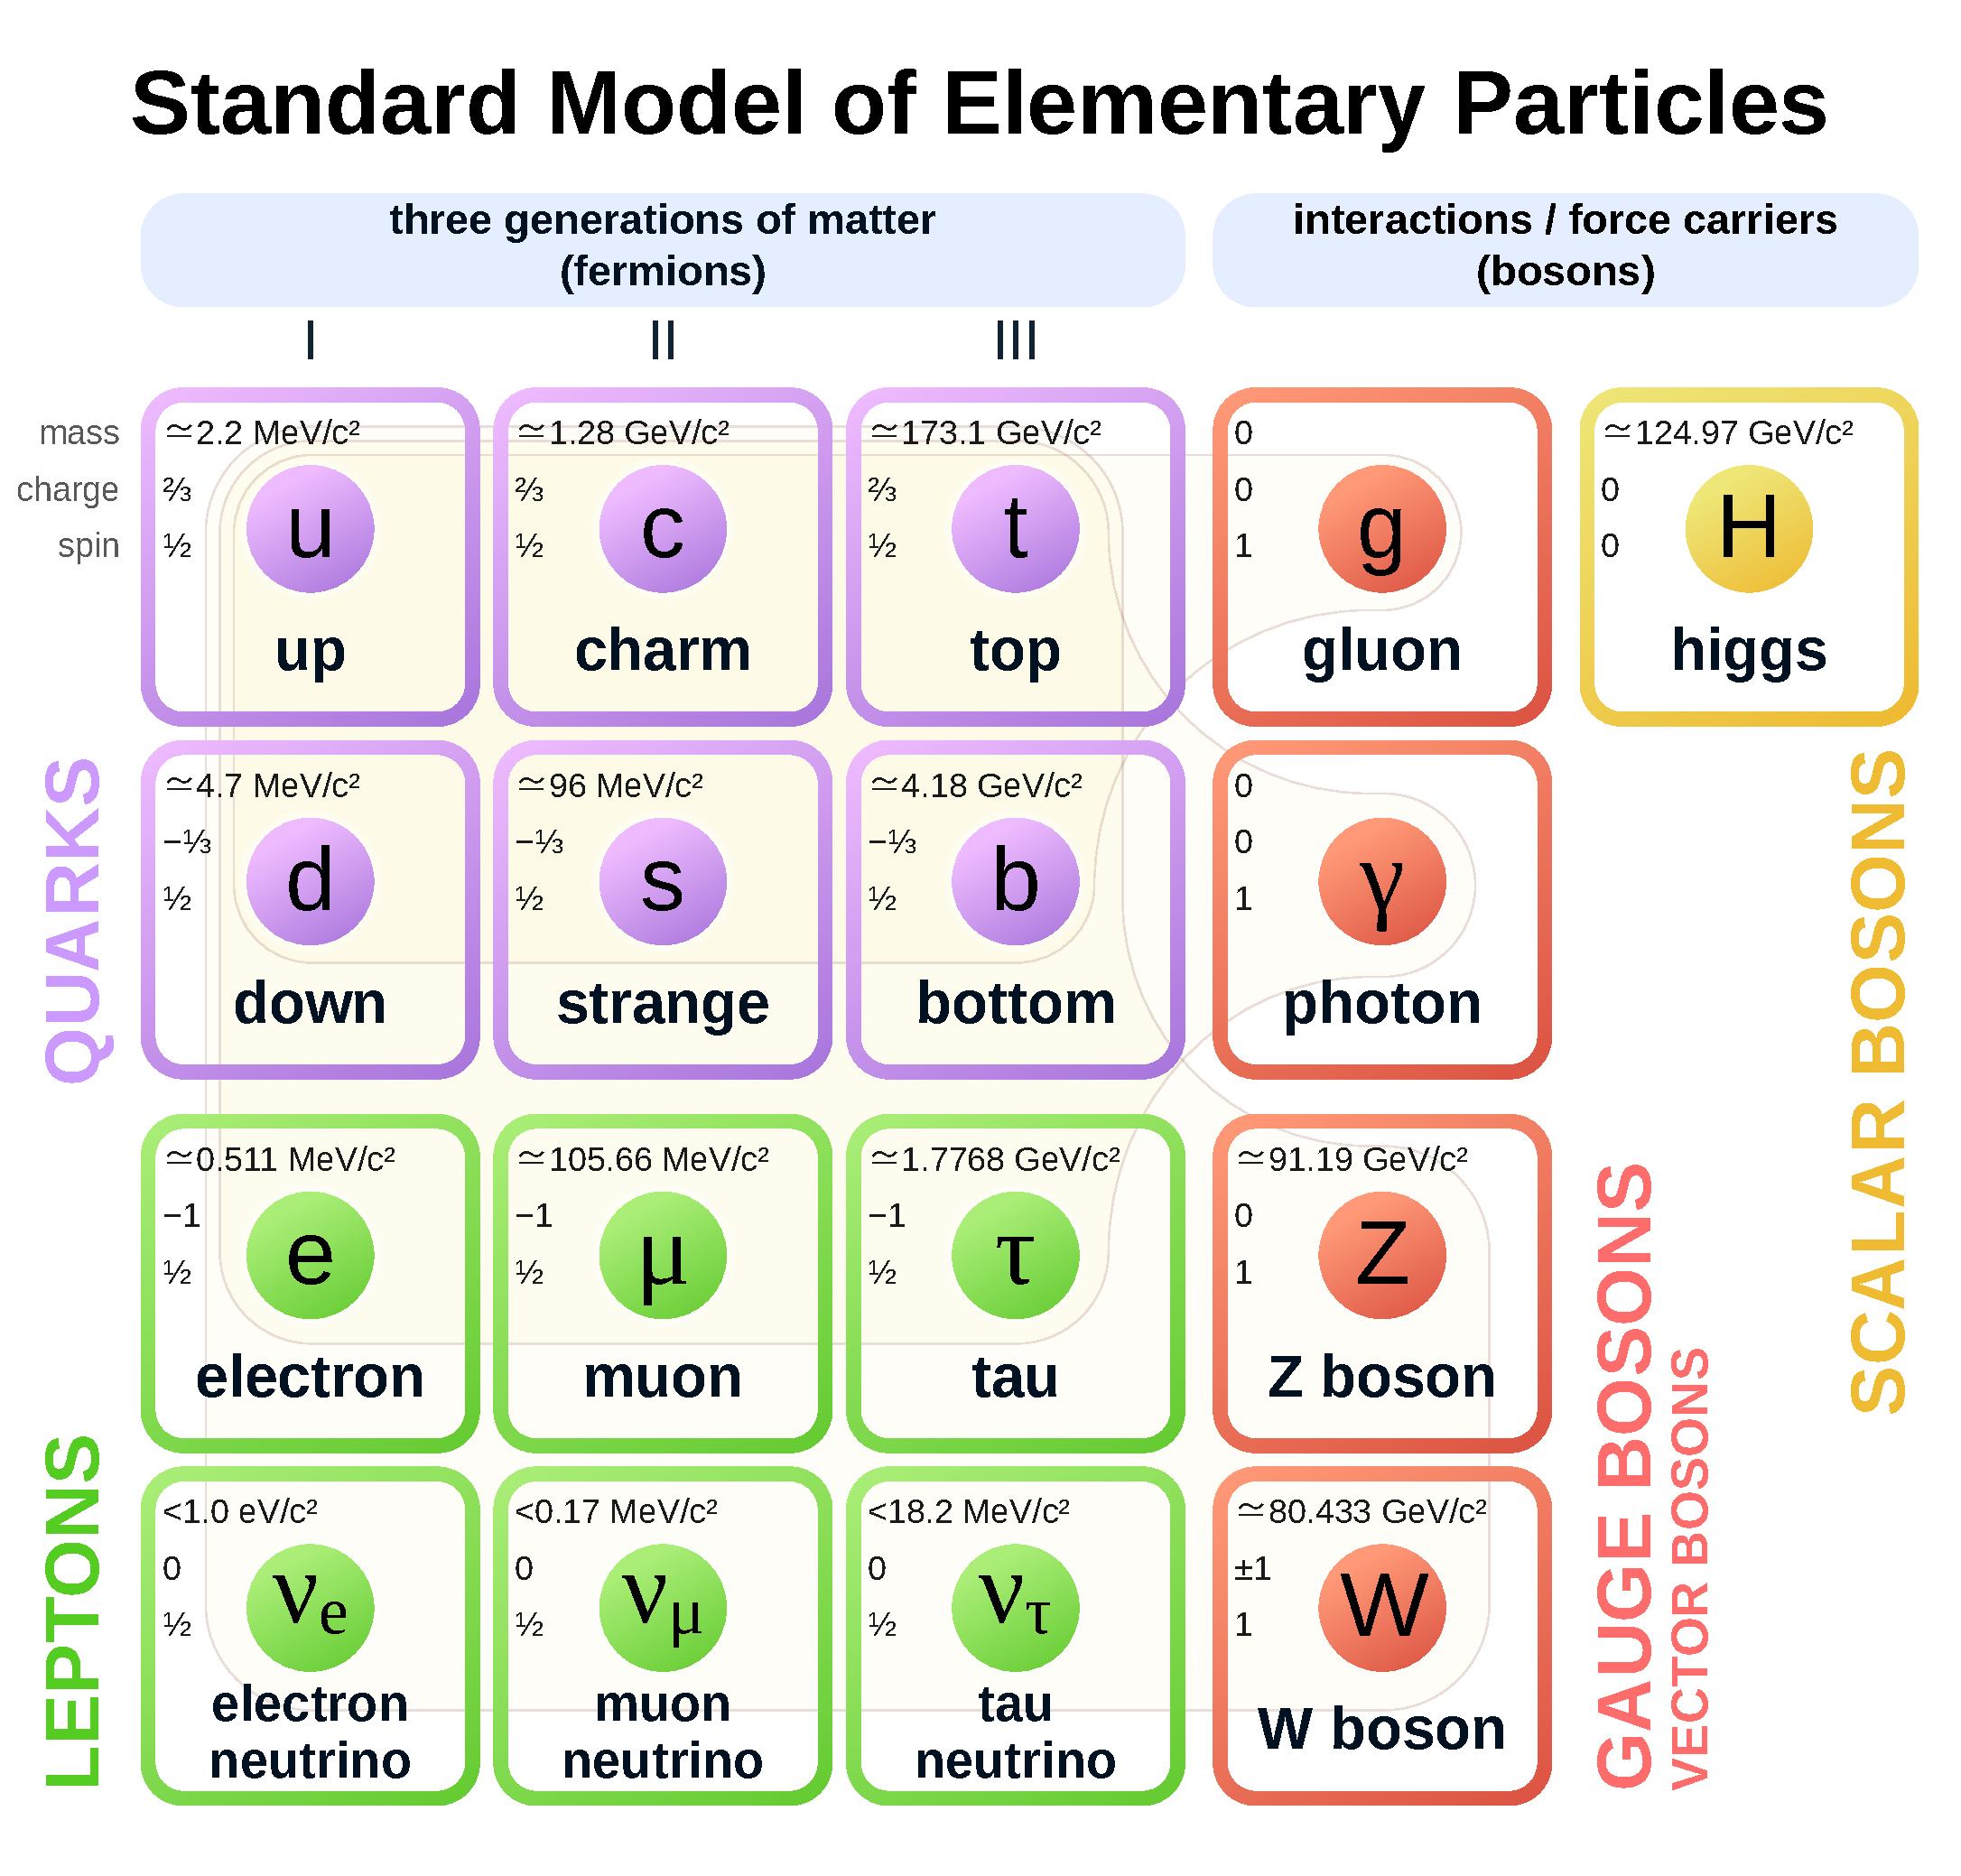
\includegraphics[width=\linewidth]{introduction/sm_particles.pdf}
        \caption{Particle content of the SM split into quarks, leptons,
        gauge bosons and scalar bosons. The columns for the fermions depict
        the three different generations. Masses, electric charge, and spin
        are given for each particle. The yellow contours indicate the coupling
        of bosons to fermions, illustrating the forces experienced by the
        fermions inside the contour. Figure reference \cite{SM_figure}.}
        \label{fig:SM_particles}
    \end{figure}
    The interactions of these fields are governed by the SM Lagrangian
    \footnote{technically Lagrangian density but we use the terms
    Lagrangian and Lagrangian density interchangeably}
    which can be written as
    \begin{equation}\label{eqn:L_SM}
        \mathcal{L}_{\mathrm{SM}} = \mathcal{L}_{\mathrm{gauge}} + \mathcal{L}_{\mathrm{fermion}} + \mathcal{L}_{\mathrm{Higgs}} + \mathcal{L}_{\mathrm{Yukawa}} + \mathcal{L}_{\mathrm{GF}} + \mathcal{L}_{\mathrm{ghost}} \, ,
    \end{equation}
    where $\mathcal{L}_{\mathrm{gauge}}$ describes the gauge fields,
    $\mathcal{L}_{\mathrm{fermion}}$ describes how fermions interact with
    gauge fields as well as their kinetic terms,
    $\mathcal{L}_{\mathrm{Higgs}}$ describes the Higgs field,
    $\mathcal{L}_{\mathrm{Yukawa}}$ describes the interaction between the Higgs
    field and fermions,
    $\mathcal{L}_{\mathrm{GF}}$ is a gauge fixing term,
    and $\mathcal{L}_{\mathrm{ghost}}$ is a ghost term.
    The last two terms are required to remove unphysical degrees of freedom
    when gauge fixing the theory.
    All terms in the SM Lagrangian are invariant under local transformations
    of the gauge group (\ref{eqn:SM_gauge}).

    In the following section we will focus on the gauge, fermion, gauge-fixing
    and ghost Lagrangian terms in the framework of QCD as that will be the
    most relevant sector for this thesis. The remaining terms are discussed at
    length in standard reference texts \cite{Peskin:1995ev,Schwartz:2014sze,Romao:2012pq}.


\section{Introduction to quantum chromodynamics}
\begin{itemize}
    \item QCD is the quantum field theory describing the strong
    interaction between quarks and gluons. It is a non-abelian
    gauge theory with gauge group SU(3).
    \item Write down the Lagrangian of QCD and define all the
    terms (field strength tensor, quark fields, group generators,
    structure constants, coupling constants.)
    \item Begin to talk about how Feynman rules can be used
    to represent the interactions that you can derive from
    the Lagrangian.
\end{itemize}
    Quantum chronodynamics (QCD) is the sector of the SM that
    describes the strong interaction. 
    QCD is a non-abelian gauge theory with gauge group
    $\mathrm{SU}(3)_{C}$ where the charge is named colour.
    The gauge and fermion part of the QCD Lagrangian is
    \begin{equation}\label{eqn:L_QCD}
        \mathcal{L}_{\mathrm{QCD}} = -\dfrac{1}{4}F^{a}_{\mu\nu}F^{a, \, \mu\nu}
        + \sum_{f} \bar{\psi}_{i}^{f}(\mathrm{i}\slashed{D}_{ij} - \delta_{ij}m_{f})\psi_{j}^{f} \, ,
    \end{equation}
    where twice repeated indices are summed over.
    The fields $\psi_{i}^{(f)}$ ($\bar{\psi}_{i}^{f}$) are the fermions (antifermions),
    representing quarks (antiquarks) with flavours $f$: 
    up $u$, down $d$, strange $s$, charm $c$, top $t$, and bottom $b$,
    with masses $m_{f}$. They transform under the fundamental
    representation with indices $i, j \in \{1, 2, 3\}$, named colour indices.
    The gauge fields $A^{a}_{\mu}$, corresponding to gluons, 
    appear in the quark covariant derivative
    \begin{equation}\label{eqn:covariant_deriv}
        (D_{\mu})_{ij} = \delta_{ij}\partial_{\mu} - ig_{\mathrm{s}}T^{a}_{ij}A^{a}_{\mu} \, ,
    \end{equation}
    and the gauge field strength tensor
    \begin{equation}\label{eqn:F_munu}
        F^{a}_{\mu\nu} = \partial_{\mu}A^{a}_{\nu} - \partial_{\nu}A^{a}_{\mu} + g_{\mathrm{s}} f^{abc}A^{b}_{\mu}A^{c}_{\nu} \, .
    \end{equation}
    Gauge fields transform under the adjoint representation, meaning
    the adjoint indices $a,b,c \in \{1,...,8\}$. $T^{a}_{ij}$ are the
    group generators in a fundamental representation. In SU(3) it is
    common to write the group generators as
    \begin{equation}\label{eqn:group_generators}
        T^{a}_{ij} = \dfrac{1}{2}\lambda^{a}_{ij}
    \end{equation}
    where $\lambda^{a}_{ij}$ are the Gell-Mann matrices \cite{Gell-Mann:1962yej}.
    The generators of the group have to obey the Lie algebra
    \begin{equation}\label{eqn:lie_algebra}
        [T^{a}, T^{b}] = \mathrm{i}f^{abc}T^{c} \, ,
    \end{equation}
    where $f^{abc}$ are the structure constants of SU(3).
    The gauge coupling of the group $g_{\mathrm{s}}$
    is a dimensional free parameter of the theory, usually
    written as
    \begin{equation}\label{eqn:alpha_s}
        \alpha_{\mathrm{s}} = \dfrac{g_{\mathrm{s}}^{2}}{4\pi} \, ,
    \end{equation}
    for reasons which will become clear when we introduce
    scattering amplitudes.

\subsection{Running coupling}
\begin{itemize}
    \item Strength of the coupling depends on the energy
    that the process occurs at. This is known as the running
    of the coupling.
    \item The value of $\alpha_{s}$ is usually quoted
    at the mass of the Z boson.
    \item In QCD the evolution of $\alpha_{s}$ is governed
    by the renormalisation group equation (Callan-Symanzik
    $\beta$ function). The coefficients of this function
    are known to many loops.
    \item Asymptotic freedom is a property of non-abelian
    gauge groups and this discovery won a Nobel prize.
\end{itemize}
\subsection{Scattering amplitudes}
\begin{itemize}
    \item S-matrix/Transition matrix
    \item Make the link between Feynman diagrams and
    scattering amplitudes/matrix elements. The sum
    of all Feynman diagrams you can draw for a particular
    process is the matrix element.
    \item Explicitly state how the QCD Feynman rules are
    derived and have the corresponding diagrams.
    \item Explain how you can basically join these
    Feynman rules into a diagram which represents a
    convenient way to calculate interactions between
    particles.
    \item Introduce the concept of loop amplitudes here,
    which naturally leads onto divergences.
    \item UV divergences lead to the introduction of
    dimensional regularisation and also to renormalisation
    of fields to make them represent physical quantities.
    The main scheme that people use is the modified minimal
    subtraction scheme.
\end{itemize}
\section{Experiments and Phenomonology}
\subsection{Observables}
\begin{itemize}
    \item Experiments do not measure single particles,
    they measure hadrons which is far from the collision
    of protons.
    \item Factorisation of hard and soft scales leads
    to the concepts of PDFs (DGLAP equation), partonic
    cross-sections (Feynman diagrams), parton showers,
    and hadronisation.
    \item Link back to matrix elements and how they
    are integrated to give you cross-sections which
    can be compared with experiments.
    \item Probably need to talk about infrared safe
    observables and jets.
\end{itemize}
\section{Monte Carlo event generator overview}
\subsection{Event unweighting}
\begin{itemize}
    \item MC generators are the main tools that
    people use to compare with experimental data.
    There are many groups that have their own tool.
    \item The usage of MC tools came about because
    the multi-dimensional phase-space integrals
    are too complex to do analytically.
    \item This doesn't mean that they only do
    the integrals, the event generators basically
    contain all the tools from phase-space generation
    to matrix element evaluation, to parton showers
    to hadronisation.
    \item Have a look at Katherina thesis to see
    how much I can skip because only really want to
    introduce unweighting. Probably along the lines
    of event weight is statistically sampled vs
    what they measure in real life. Therefore we need
    to unweight events.
\end{itemize}
\end{document}